\documentclass[lecture_notes.tex]{subfiles}

\begin{document}

\notestitle{Session 4}{Matrix Product States for Spin Chains}%
  {mps\_quantum\_magnets.ipynb}{exact diagonalization of the Heisenberg model (Session 2)}

\section*{Contents and goals}
Last session we solved the Heisenberg model exactly, by brute-force diagonalization, and it
worked beautifully: gaps, level crossings, correlators, all of it came out of the numerics with
no approximation at all. But we also ran straight into a wall. The Hilbert space of $L$
spin-$\tfrac12$'s has dimension $2^L$, and that number simply refuses to be tamed: by around
$L\sim 20$ spins, even a very good computer has run out of memory, and we are nowhere near the
thermodynamic limit where the genuinely interesting physics, quantum phase transitions,
fractionalization, the emergence of gaps, actually lives. So the question for today is very
concrete: is there a way to represent the many-body wavefunction that does not cost us
exponentially much, at least for the states we actually care about? The answer is yes, and it
goes by the name of matrix product states (MPS), the simplest member of the broader family of
tensor network methods. We will see why this representation is efficient, what makes it work so
well specifically in one dimension, how to tell numerically whether we trust it, and then we will
spend the second half of the session simply redoing session 2's Heisenberg-model story, but now
at $40$ to $100+$ spins, large enough to see thermodynamic-limit physics we could only guess at
before.

\section*{Learning outcomes}
By the end of this session, you should be able to:
\begin{itemize}[nosep]
  \item Explain why the matrix product state ansatz compresses an exponentially large
    wavefunction into a cost that is linear in $L$ and quadratic in the bond dimension $\chi$.
  \item Use entanglement entropy and the area law to justify why matrix product states work well
    in one dimension, and where they are expected to fail (2D, volume-law states).
  \item Assess the convergence of a variational MPS calculation using energy fluctuations, and use
    entanglement entropy as a diagnostic for a quantum phase transition.
  \item Run MPS calculations at $40$--$100+$ spins to distinguish the gapless spin-$\tfrac12$
    Heisenberg chain from the gapped, fractionalized spin-$1$ Haldane phase.
\end{itemize}

\section{From an exponential wavefunction to a matrix product state}

\subsection{Tensor networks as data compression}
Let us set the stage with an analogy before we write down any equations. Imagine you have a
high-resolution photograph and you want to store it using much less memory. You do not throw away
information at random; you exploit the fact that real photographs are highly structured, nearby
pixels are correlated with each other, and a compressed representation (think of a JPEG) can
reproduce something visually indistinguishable from the original using a small fraction of the
raw pixel count. Tensor networks do exactly the same thing, but for quantum many-body
wavefunctions. The ``raw pixels'' are the $2^L$ complex coefficients of the wavefunction in the
computational basis; the ``compression algorithm'' is a particular way of factorizing those
coefficients into small pieces, and the parameter that controls how aggressive the compression is
will turn out to be something called the \textbf{bond dimension}. The whole content of this
section is making that analogy precise.

\subsection{The formal matrix product state ansatz}
For a chain of $L$ spins, each with $d$ local states ($d=2$ for spin-$\tfrac12$, $d=3$ for
spin-$1$, and so on), an arbitrary wavefunction is
\begin{equation}
  \ket{\Psi} = \sum_{s_1,\ldots,s_L} C(s_1,\ldots,s_L)\, \ket{s_1}\otimes\cdots\otimes\ket{s_L},
  \label{eq:generalwf}
\end{equation}
and specifying $\ket{\Psi}$ exactly means specifying all $d^L$ numbers $C(s_1,\ldots,s_L)$
independently. The matrix product state ansatz makes a very specific proposal for how to generate
these coefficients without storing them one by one: for every site $n$ and every local state
$s_n$, introduce a matrix $M_n^{s_n}$, and write
\begin{equation}
  C(s_1,\ldots,s_L) = M_1^{s_1} M_2^{s_2} \cdots M_L^{s_L}.
  \label{eq:mpsansatz}
\end{equation}
For open boundary conditions, $M_1^{s_1}$ is a $1\times\chi_1$ row vector and $M_L^{s_L}$ is a
$\chi_{L-1}\times 1$ column vector, so the whole chain of matrix products in
Eq.~\eqref{eq:mpsansatz} collapses down to a single number, exactly as it must for $C$ to be a
scalar coefficient. The internal matrices $M_n^{s_n}$ are $\chi_{n-1}\times \chi_n$, and the
integer $\chi$ (we will mostly take it uniform along the chain) is the \textbf{bond dimension}: it
is the one knob that controls how much this ansatz can represent, and it is going to be the
central character of this whole session.

\begin{figure}[H]
  \centering
  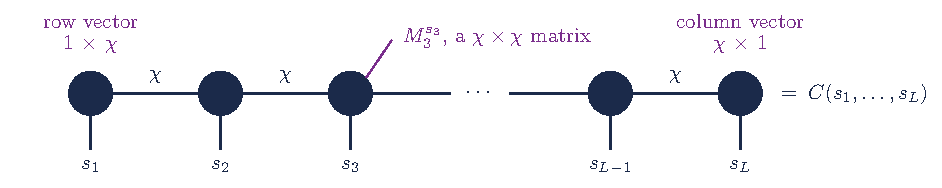
\includegraphics[width=0.90\textwidth]{figures/mps_chain.pdf}
  \caption{The matrix product state of Eq.~\eqref{eq:mpsansatz} drawn as a tensor network. Each
    site carries one tensor $M_n^{s_n}$, with a vertical \emph{physical} leg running over the $d$
    local states of that site and horizontal \emph{bond} legs of dimension $\chi$ joining it to
    its neighbors. Joining two legs means summing over the shared index, so contracting the
    horizontal legs from left to right is precisely the matrix product of
    Eq.~\eqref{eq:mpsansatz}. The two end tensors carry a single bond leg each, a row vector and
    a column vector, which is why the whole contraction collapses to one number.}
  \label{fig:mps-chain}
\end{figure}

Let us count parameters, because this is really the whole point. Storing $C(s_1,\ldots,s_L)$
directly costs us $d^L$ numbers, exponential in $L$. Storing the matrices $\{M_n^{s_n}\}$ instead
costs us
\begin{equation}
  N_{\mathrm{MPS}} \sim L\, d\, \chi^2,
  \label{eq:paramcount}
\end{equation}
which is \emph{linear} in the system size $L$ and only quadratic in the bond dimension $\chi$. So
if we can get away with representing the states we care about at some fixed, moderate $\chi$, we
have turned an exponential problem into a polynomial one. This raises the natural
question: is it actually true that the states we care about, ground states and low-lying excited
states of local Hamiltonians, can be captured this way with a $\chi$ that stays modest as $L$
grows? We will answer this properly once we introduce entanglement entropy in
Section~\ref{sec:entanglement}, but the short answer, which is really the whole reason this course
has a Session 4, is: yes, in one dimension.

\subsection{Cost: exact diagonalization versus matrix product states}
It is worth just looking at what this buys us in practice before we justify it theoretically. If
we solve the Heisenberg chain $\Ham_{\mathrm{Heis}} = J\sum_n \vb S_n\cdot\vb S_{n+1}$ by exact
diagonalization, the time to find the ground state grows exponentially with $L$, simply because we
are manipulating vectors and matrices of size $2^L$. If instead we solve it variationally over the
matrix product state ansatz of Eq.~\eqref{eq:mpsansatz}, at fixed bond dimension the cost grows
close to linearly in $L$. The two curves cross somewhere around $L\sim 14$--$16$: below that,
exact diagonalization is actually faster (there is no point using a variational method when the
exact answer is cheap), but above it, matrix product states win, and they keep winning by an
ever-growing margin. Concretely, systems of $50$, $70$, even $80$ spins become tractable on a
laptop, in seconds, while exact diagonalization would need more memory than exists on the
largest supercomputers once you pass $L\sim 40$--$50$. That gap in scaling, exponential versus
polynomial, is the entire reason this session exists.

\begin{notebook}
Sections ``Energy of the Heisenberg model as a function of the system size'' and ``Near lineal
scaling with system size with matrix product states.'' Plot the ground-state energy per site
against $L$ and see it converge toward a thermodynamic-limit value; check it against the exact
Bethe-ansatz result $e_0 = J\big(\tfrac14-\ln2\big)\approx-0.4431J$ as an independent convergence
check. Then time exact diagonalization against the matrix product state solver as you increase
$L$, and locate for yourself the crossover system size beyond which the tensor network method
becomes the only game in town.
\end{notebook}

\section{How good is the variational state? Convergence diagnostics}
Matrix product states are a variational ansatz: we are not solving the Schr\"odinger equation
exactly, we are searching for the best approximation to the ground state (or an excited state)
within the family of states described by Eq.~\eqref{eq:mpsansatz} at some fixed $\chi$. This
immediately raises a practical question we did not have to worry about with exact diagonalization:
how do we know, without knowing the exact answer, whether our variational state is actually good?

\subsection{Energy fluctuations}
Suppose our solver has converged to some normalized state $\ket{\Omega}$, with energy
$E_\Omega = \expval{\Ham}{\Omega}$. If $\ket{\Omega}$ happened to be an exact eigenstate of
$\Ham$, then $\Ham\ket{\Omega} = E_\Omega\ket{\Omega}$ and the variance of the energy,
\begin{equation}
  (\Delta E)^2 \equiv \expval{\Ham^2}{\Omega} - \expval{\Ham}{\Omega}^2,
  \label{eq:varH}
\end{equation}
would vanish identically. So a natural diagnostic is: compute $(\Delta E)^2$ using only the
variational state itself, no knowledge of the true ground state required, and check how close it
is to zero. Let us make this quantitative. Write $\ket{\Omega}$ as mostly the true ground state
$\ket{0}$ with a small admixture $\varepsilon$ of the first excited state $\ket{1}$,
\begin{equation}
  \ket{\Omega} = \sqrt{1-\varepsilon^2}\,\ket{0} + \varepsilon\,\ket{1}, \qquad \varepsilon\ll 1.
\end{equation}
A short calculation (expand $\expval{\Ham}{\Omega}$ and $\expval{\Ham^2}{\Omega}$ to
$\Order{\varepsilon^2}$ using $\Ham\ket{0}=E_0\ket{0}$, $\Ham\ket{1}=E_1\ket{1}$) gives
\begin{equation}
  E_\Omega - E_0 = \varepsilon^2(E_1-E_0), \qquad
  (\Delta E)^2 = \varepsilon^2(E_1-E_0)^2 + \Order{\varepsilon^4}.
  \label{eq:varHresult}
\end{equation}
Two things follow immediately, and both are exactly what makes this diagnostic so useful. First,
$(\Delta E)^2 \to 0$ if and only if $\varepsilon\to 0$, i.e.\ if and only if $\ket{\Omega}$
converges onto a true eigenstate: the fluctuation is a perfectly good stand-in for the (unknown)
distance to the exact answer. Second, comparing the two relations in
Eq.~\eqref{eq:varHresult} tells us that $(\Delta E)^2 \approx (E_\Omega - E_0)(E_1-E_0)$, so the
energy fluctuation is simultaneously telling us both how contaminated our state is by an excited
state \emph{and} roughly what the gap to that excited state is. In practice we watch
$(\Delta E)^2$ as we increase the bond dimension $\chi$: it should decrease monotonically and
eventually flatten out near machine precision once $\chi$ is large enough for the physics at hand.

\subsection{Bond dimension and excited states}
Everything we just said for the ground state applies unchanged to any targeted eigenstate: an
excited-state solver also converges toward some $\ket{\Omega_k}\to\ket{k}$ as $\chi$ increases, and
we can monitor the same energy fluctuation, Eq.~\eqref{eq:varH}, evaluated on $\ket{\Omega_k}$. What
changes is \emph{how fast} this convergence happens. Higher excited states are, generically, more
entangled than the ground state (they explore a larger portion of the Hilbert space, and, as we
will see in Section~\ref{sec:entanglement}, entanglement is exactly what a finite bond dimension
struggles to capture), so they need larger $\chi$ before their energy fluctuation collapses toward
zero. This is a completely generic feature of tensor network calculations: the ground state
converges first and fastest, and each successive excited state needs a bit more bond dimension to
catch up.

\begin{notebook}
Sections ``The role of the bond dimension'' and ``The role of bond dimension in excited states.''
Plot the ground-state energy and its fluctuation, Eq.~\eqref{eq:varH}, against $\chi$ for the
Heisenberg chain, and watch the fluctuation collapse as $\chi$ grows. Then repeat for several
excited states at once and confirm that higher-lying states need larger $\chi$ to converge to the
same fluctuation tolerance.
\end{notebook}

\section{Low-energy excitations and level crossings}
Before we build up the full entanglement-entropy machinery, it is worth seeing what matrix product
states buy us physically, using the same first excited state we just discussed as a diagnostic.

Take the Heisenberg chain and compute the matrix element $\bra{0}S_n^x\ket{1}$ between the ground
state and the first excited state, as a function of the site $n$ where we act with the spin
operator. Physically, this tells us the amplitude for creating the lowest-energy spin excitation
at site $n$. For the spin-$\tfrac12$ chain, this profile looks like the ground-state wavefunction
of a particle in a box: maximal amplitude at the center of the chain, decaying smoothly toward
both edges. This is not a coincidence: it is the same lowest-triplet magnon that dispersed as a
plane wave on Session 2's periodic dimer and small chains, now standing on an \emph{open} chain,
where the boundaries force it into a standing wave with a node at each edge instead of a running
wave. This is exactly the behavior of a delocalized, bulk spin excitation, and it is our
first hint that the low-energy physics of the spin-$\tfrac12$ chain lives in the bulk. We will
come back to a sharp contrast with this profile, for spin-$1$, once we have enough system size to
make the comparison convincing (Section~\ref{sec:fractionalization}).

The other natural thing to track is how the ground state itself changes as we turn on a magnetic
field, $\Ham = J\sum_n \vb S_n\cdot\vb S_{n+1} - B\sum_n S_n^z$. Since $\sum_n S_n^z$ commutes with
the exchange term, applying $B$ never mixes eigenstates of $\Ham|_{B=0}$; it simply relabels their
energies by $-B\times(\text{total }S^z)$, and different total-$S^z$ sectors cross each other as $B$
increases. For $L=2$ there is exactly one such crossing, from the $S=0$ singlet to the $S=1$
triplet; for $L=4$ there are two, $S=0\to S=1\to S=2$; and as we grow $L$, more and more crossings
appear, packed closer and closer together in $B$. This is a very direct, numerically clean way of
seeing that the spin-$\tfrac12$ Heisenberg chain is gapless in the thermodynamic limit: the
staircase of crossings becomes a smooth ramp as $L\to\infty$, meaning there exist excitations
arbitrarily close in energy to the ground state at any nonzero $B$.

\begin{notebook}
Sections ``Low energy excitations of a Heisenberg model'' and ``Level crossings as a function of
the magnetic field with matrix product states.'' Reproduce the particle-in-a-box matrix-element
profile, and separately track the ground-state total spin as a function of $B$ for $L=2,4,10,30$:
watch the discrete staircase of session 2 smooth out into what will look like a continuous ramp
once $L$ is large enough.
\end{notebook}

\section{Entanglement entropy: why matrix product states work in one dimension}
\label{sec:entanglement}
We have used the matrix product state ansatz for two sections now without ever justifying it. Let
us finally do that properly, because the justification is also what tells us, precisely, when this
whole approach is going to fail.

\subsection{Separable versus entangled states}
Take a bipartition of our system into two regions, $A$ and $B$ (think of $A$ as the left half of
the chain and $B$ as the right half). We say a state $\ket{\Psi}$ is \textbf{separable} if it
factorizes as a simple tensor product,
\begin{equation}
  \ket{\Psi} = \ket{\phi}_A \otimes \ket{\chi}_B,
\end{equation}
for some states $\ket{\phi}_A$, $\ket{\chi}_B$ living purely on $A$ and purely on $B$. A basis
state like $\ket{\up\dn}$ is trivially of this form, $\ket{\up}_A\otimes\ket{\dn}_B$; so, less
obviously but just as directly, is a state where every spin points along $x$, since
$\ket{\to}\otimes\ket{\to} = \tfrac12(\ket{\up}+\ket{\dn})\otimes(\ket{\up}+\ket{\dn})$ is still a
product. Every classical configuration, in fact every state you can write down without any
correlation between $A$ and $B$, is separable in this sense. But now take the two-site singlet we
met already in Session 1,
\begin{equation}
  \ket{\Psi_{\mathrm{singlet}}} = \frac{1}{\sqrt2}\Big(\ket{\up\dn} - \ket{\dn\up}\Big).
\end{equation}
No choice of $\ket{\phi}_A$, $\ket{\chi}_B$ reproduces this: try to write it as a product and you
immediately find you need two different terms with opposite relative sign, which a single product
cannot generate. We call such a state \textbf{entangled}. This is precisely the distinction that
separates classical states from genuinely quantum ones, and we need a way to quantify \emph{how}
entangled a state is, not just whether it is or is not.

\subsection{The reduced density matrix and the von Neumann entropy}
Given the full density matrix $\rho = \ket{\Psi}\bra{\Psi}$, define the \textbf{reduced density
matrix} of subsystem $A$ by tracing out everything in $B$,
\begin{equation}
  \rho_A \equiv \operatorname{Tr}_B\rho.
\end{equation}
The \textbf{entanglement entropy} across the cut is then just the ordinary von Neumann entropy of
$\rho_A$,
\begin{equation}
  S_A \equiv -\operatorname{Tr}\big[\rho_A \ln \rho_A\big].
  \label{eq:vonNeumann}
\end{equation}
If $\ket{\Psi}$ is separable, $\rho_A = \ket{\phi}\bra{\phi}$ is a rank-one projector, its only
nonzero eigenvalue is $1$, and $S_A = -1\ln 1 = 0$. If $\ket{\Psi}$ is the singlet, a direct
computation of $\rho_A$ (trace out site $B$) gives $\rho_A = \tfrac12\mathbb{1}$, with two equal
eigenvalues $\tfrac12,\tfrac12$, so $S_A = -2\times\tfrac12\ln\tfrac12 = \ln 2$, the maximal
possible entropy for a single spin-$\tfrac12$. So $S_A$ really does interpolate smoothly between
``no entanglement'' and ``maximal entanglement,'' exactly as we want.

\subsection{Schmidt decomposition: the bond dimension bounds the entanglement}
Now let us connect this directly to the matrix product state ansatz. Cut the chain at bond $n$,
between sites $n$ and $n+1$. Any state can be written, via a singular value decomposition of its
coefficient tensor reshaped as a matrix between the left block $(1,\ldots,n)$ and the right block
$(n+1,\ldots,L)$, in the \textbf{Schmidt form}
\begin{equation}
  \ket{\Psi} = \sum_{\alpha=1}^{r} \lambda_\alpha \ket{\alpha}_A \otimes \ket{\alpha}_B,
  \qquad \sum_\alpha \lambda_\alpha^2 = 1,
  \label{eq:schmidt}
\end{equation}
with $\ket{\alpha}_A$, $\ket{\alpha}_B$ orthonormal on each side and $r$ the Schmidt rank. For a
generic state, $r$ can be as large as $d^{\min(n,L-n)}$, exponential in the block size. But for a
matrix product state built as in Eq.~\eqref{eq:mpsansatz}, the sum over the bond index at position
$n$ runs only over $\chi_n$ values by construction, so the coefficient tensor manifestly
factorizes through a $\chi_n$-dimensional index: the Schmidt rank at that cut can be at most
$\chi_n$. Plugging the Schmidt form into Eqs.~\eqref{eq:vonNeumann} gives
$\rho_A = \sum_\alpha \lambda_\alpha^2 \ket{\alpha}\bra{\alpha}$, so
\begin{equation}
  S_A = -\sum_{\alpha=1}^{r} \lambda_\alpha^2 \ln \lambda_\alpha^2 \;\le\; \ln r \;\le\; \ln \chi_n,
  \label{eq:arealawbound}
\end{equation}
with equality in the last step exactly when all $\chi_n$ Schmidt weights are equal,
$\lambda_\alpha^2 = 1/\chi_n$. This is the single most important equation in this session:
\emph{the bond dimension caps the entanglement entropy the ansatz can represent}. If the state we
are after has entanglement entropy $S_A$ across some cut, we need at least $\chi \gtrsim e^{S_A}$
there to capture it. So the entire question of whether matrix product states are a good idea for a
given problem reduces to: how does $S_A$ behave as we grow the system?

\begin{figure}[H]
  \centering
  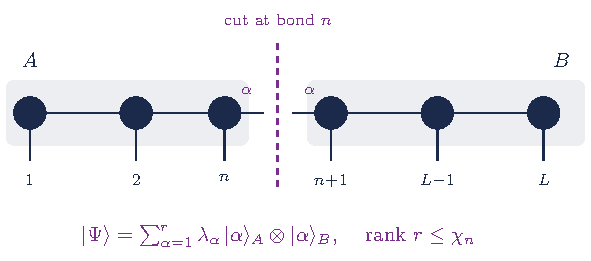
\includegraphics[width=0.70\textwidth]{figures/schmidt_cut.pdf}
  \caption{The Schmidt decomposition of Eq.~\eqref{eq:schmidt} read directly off a matrix product
    state. Cutting the chain at bond $n$ separates it into blocks $A$ and $B$ and exposes the
    single bond index $\alpha$ that joined them. Since that index takes only $\chi_n$ values by
    construction, the sum in Eq.~\eqref{eq:schmidt} can run over at most $\chi_n$ terms, the
    Schmidt rank obeys $r\le\chi_n$, and the entropy across the cut obeys the bound of
    Eq.~\eqref{eq:arealawbound}. Everything the two halves of the chain know about each other has
    to pass through that one index.}
  \label{fig:schmidt-cut}
\end{figure}

\subsection{The area law, and why one dimension is cheap}
Here is the key physical fact. For the ground state of a \emph{gapped}, local, one-dimensional
Hamiltonian, correlations decay exponentially beyond some correlation length $\xi$, and it turns
out (this is the celebrated area-law theorem for 1D gapped systems) that $S_A$ \emph{saturates} to
an $L$-independent constant as soon as the block $A$ is a few $\xi$ away from both its boundary and
the far end of the chain. Only the physics living within $\sim\xi$ of the cut contributes to the
entanglement; everything deep in the interior of $A$ or $B$ is irrelevant to it. For a
\emph{gapless}, critical chain there is no finite $\xi$, and conformal field theory tells us $S_A$
instead grows, but only logarithmically, $S_A \sim \tfrac{c}{3}\ln n$ for a cut in the bulk of an
infinite or periodic chain (open boundaries, which we adopt throughout this session and motivate in
Section~\ref{sec:bc}, roughly halve this to $S_A\sim\tfrac{c}{6}\ln n$). Either way, this is
enormously cheaper than the generic case: a uniformly random state in the Hilbert space (this is
Page's theorem) has $S_A$ growing linearly with the size of the smaller block, a \emph{volume law},
which would force $\chi$ to grow exponentially with system size and defeat the whole purpose of the
ansatz. Ground states of local 1D Hamiltonians are a vanishingly special corner of the full Hilbert
space, and it is precisely because they live in that corner, low or at most logarithmically growing
entanglement, that a bond dimension $\chi$ that stays modest (or grows only polynomially) as
$L\to\infty$ can capture them accurately.

A very clean way to see the saturation directly is to solve an exactly dimerized chain, where sites
are grouped into decoupled pairs, $\Ham = J\sum_k \vb S_{2k-1}\cdot\vb S_{2k}$ with no coupling
between pairs. The exact ground state is simply a product of singlets,
$\ket{\Psi} = \bigotimes_k \ket{\Psi_{\mathrm{singlet}}}_{2k-1,2k}$. Now cut this state anywhere:
every cut either falls \emph{inside} a singlet, contributing $\ln 2$ (from
Eq.~\eqref{eq:vonNeumann} above), or falls \emph{between} singlets, contributing nothing at all,
since the two halves factorize exactly there. However large a block $A$ we choose, as long as its
boundary sits between dimers, $S_A$ is either $0$ or $\ln2$ per boundary point, completely
independent of the size of $A$. This is the area law in its most transparent form: entanglement is
a property of the \emph{boundary} of the cut, not of its volume, and in one dimension a boundary is
just a point (or two, for an interior block), so it costs $\Order{1}$ no matter how big the system
gets.

\begin{notebook}
Sections ``Entanglement entropy of the ground state,'' ``Size dependence of the entanglement
entropy,'' and ``Bond dimension dependence of the entanglement entropy.'' Compute $S_A$ at every
bond of a Heisenberg chain for a few values of $\chi$, and check that increasing $\chi$ beyond
some point stops changing the profile at all: that saturation is a direct, numerical confirmation
of the bound in Eq.~\eqref{eq:arealawbound}. Then track the entanglement entropy at the central
bond as you grow $L$, and confirm it grows only very slowly, consistent with the (logarithmic, for
the gapless Heisenberg chain) area-law scaling described above.
\end{notebook}

\paragraph{Why two dimensions is expensive.} The same bond-counting argument, run in two
dimensions, gives the opposite conclusion. Tile a 2D lattice into decoupled clusters (say,
plaquettes of four spins each, fully coupled inside and disconnected between clusters) and repeat
the exercise: a rectangular block $A$ now cuts through a number of inter-cluster bonds
proportional to the \emph{perimeter} of $A$, not to a fixed number of points. Doubling the linear
size of $A$ roughly doubles the number of boundary clusters, and hence doubles $S_A$. Since a
matrix product state has to linearize the 2D lattice into an effective 1D chain (snaking through
the rows), the bond crossing the ``middle'' of that snake has to carry the entanglement of an
entire row, so $\chi$ needs to grow \emph{exponentially} with the linear dimension of the system to
keep the truncation error fixed. Matrix product states can still be used in two dimensions (this is
how some of the best available numerics for the 2D Hubbard model or frustrated triangular and
kagome-lattice antiferromagnets are obtained), but only by working on narrow cylinders and paying
for a much larger $\chi$ than a comparable 1D calculation would need. We will not pursue 2D tensor
networks further in this course; this is slides-only material, flagged here because it explains
directly why everything else in this session is specific to $d=1$.

\paragraph{Where matrix product states struggle even in 1D.} Bounded, area-law entanglement is a
property of \emph{ground states} of \emph{gapped or mildly critical, local} Hamiltonians. It fails,
and matrix product states fail along with it, in a few important situations worth knowing about
even though we will not explore them numerically here: entanglement grows \emph{linearly} in time
under quantum quench dynamics (so time evolution with matrix product states is only trustworthy up
to some maximal time set by $\chi$), highly excited states deep in the many-body spectrum typically
violate the area law entirely, and long-range interactions effectively reintroduce
higher-dimensional connectivity even in a nominally 1D chain. This is again slides-only material,
not covered in the companion notebook.

\section{Boundary conditions}
\label{sec:bc}
One more practical lesson, before we move to the physics: the choice between open and periodic
boundary conditions matters a great deal for tensor networks, even though it barely matters for
exact diagonalization (there, periodic boundary conditions just add one more coupling term to the
Hamiltonian matrix). With open boundary conditions, a bulk cut severs exactly \emph{one} bond of
the chain, so the area-law argument above applies directly. With periodic boundary conditions, the
chain is a ring, and any bipartition into two contiguous arcs severs the ring at \emph{two} points
rather than one, since the two arcs are each other's neighbors on both ends. Both cuts contribute
to the entanglement entropy across that partition, so periodic boundary conditions roughly
\emph{double} $S_A$ compared to open boundary conditions on the same chain. Doubling the entropy
means, by Eq.~\eqref{eq:arealawbound}, that we need roughly the \emph{square} of the bond dimension
to reach the same accuracy. This is why virtually every practical matrix product state calculation,
including everything else in this session, uses open boundary conditions: periodic chains are
simply much more expensive for the same physical answer.

\begin{figure}[H]
  \centering
  \begin{subfigure}[c]{0.60\textwidth}
    \centering
    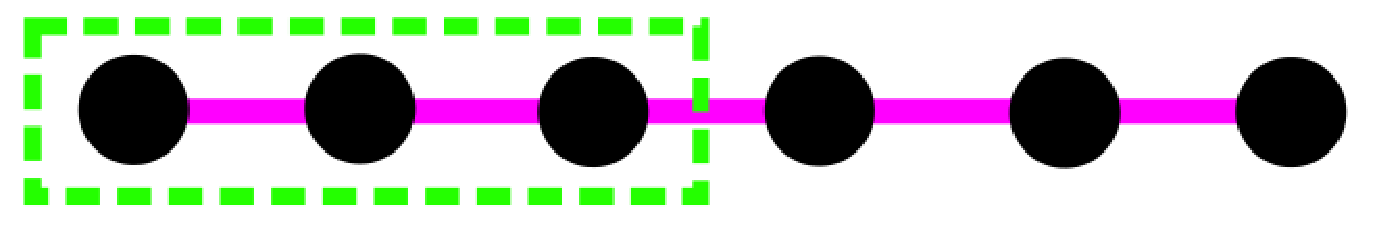
\includegraphics[width=\linewidth]{figures/mps_spin_chains/boundary_open_schematic.pdf}
    \caption{Open chain, one cut}
  \end{subfigure}\hfill
  \begin{subfigure}[c]{0.24\textwidth}
    \centering
    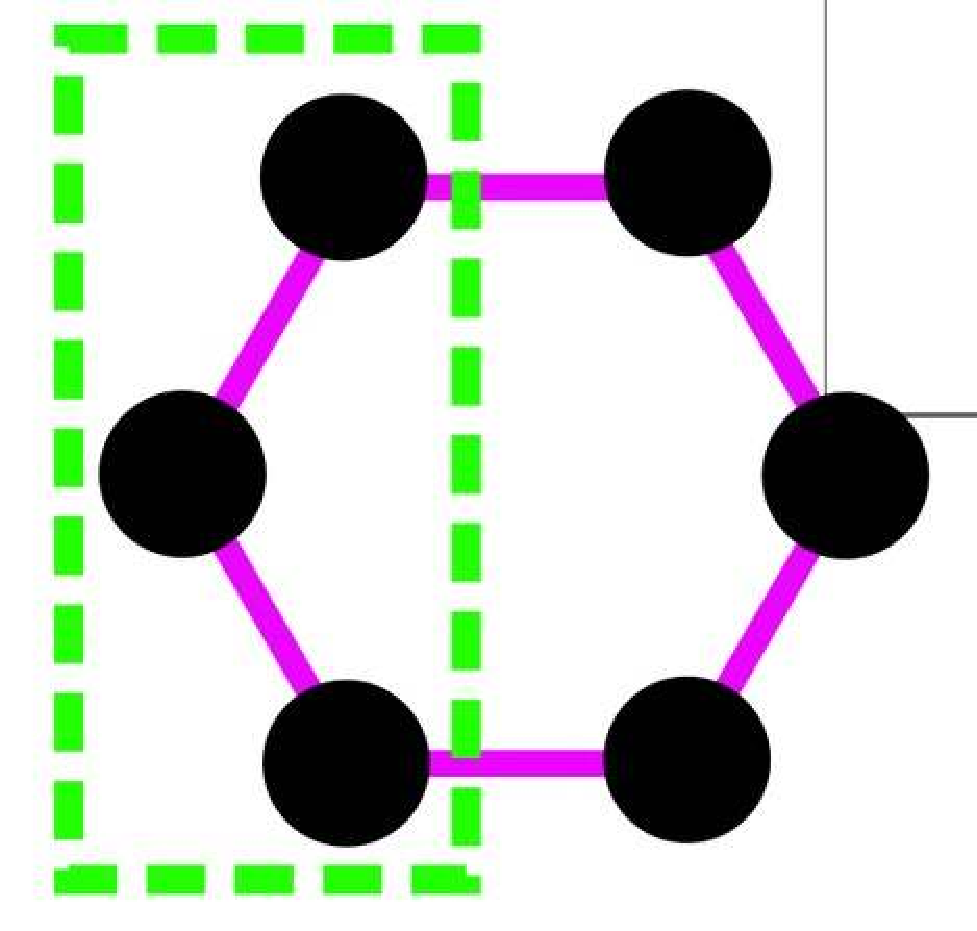
\includegraphics[width=\linewidth]{figures/mps_spin_chains/boundary_closed_schematic.pdf}
    \caption{Ring, two cuts}
  \end{subfigure}
  \caption{Why open boundaries are so much cheaper. The dashed line marks the block $A$ whose
    entanglement entropy we compute. (a) On an open chain, a contiguous block borders the rest of
    the system at a single point, so one bond is severed. (b) On a ring the same block is
    adjacent to the rest at both of its ends, so any bipartition severs two bonds and each one
    contributes, roughly doubling $S_A$. Through the bound of
    Eq.~\eqref{eq:arealawbound}, a doubled entropy costs us the \emph{square} of the bond
    dimension for the same accuracy.}
  \label{fig:boundary-cuts}
\end{figure}

\begin{notebook}
Section ``Open and closed boundary conditions.'' Compute the central-bond entanglement entropy of
the Heisenberg chain with both open and periodic boundary conditions as a function of $L$, and
check numerically that the periodic curve sits roughly at twice the open one.
\end{notebook}

\section{Entanglement entropy as a diagnostic for quantum phase transitions}

\subsection{The transverse-field Ising model}
\label{sec:tfi}
Entanglement entropy is not just a bookkeeping device for tensor network cost, it is a genuine
physical diagnostic in its own right, and nowhere is this cleaner than at a quantum phase
transition. Consider the transverse-field Ising chain,
\begin{equation}
  \Ham_{\mathrm{TFI}} = -J\sum_n S_n^z S_{n+1}^z - B_x \sum_n S_n^x.
  \label{eq:tfi}
\end{equation}
This model has two exactly solvable limits. At $B_x=0$, only the $S^zS^z$ term survives, and even
though $S^z_n$ is a quantum operator, the Hamiltonian is diagonal in the $S^z$ basis: the ground
state is the classical, fully polarized ferromagnet, $\ket{\up\up\cdots\up}$ (or its degenerate
partner $\ket{\dn\dn\cdots\dn}$). At $B_x\to\infty$, we can instead drop the exchange term entirely,
and the ground state is again classical, this time fully polarized along $x$,
$\ket{\to\to\cdots\to}$. Both limits are separable product states, so by
Eq.~\eqref{eq:vonNeumann} their entanglement entropy is exactly zero. Somewhere in between,
$\Ham_{\mathrm{TFI}}$ must interpolate between these two very different classical orders, and it
does so through a genuine quantum phase transition. (The exact solution of this model comes from
mapping spins onto free fermions via a Jordan-Wigner transformation, a construction we will meet
properly in Session 5; it places the critical point, for the normalization used here, at
$B_x = J/2$.)

\subsection{The entanglement peak and the order parameter}
Since both classical limits have zero entanglement entropy, and the state in between them is
genuinely quantum (a superposition that cannot be reduced to a single classical spin
configuration), $S_A$ has to rise away from zero somewhere in the middle and come back down, and
the natural guess is that it peaks exactly at the phase transition. This is precisely what the
numerics show: computing $S_A$ at the central bond of a long chain as a function of $B_x/J$, we
see it vanish at both $B_x=0$ and $B_x\to\infty$, with a pronounced maximum sitting right at the
critical point. For a chain of $\sim 100$ spins, close enough to the thermodynamic limit, that peak
sits at $B_x/J = 0.5$, exactly the exact value quoted above.

We can cross-check this against a completely independent, and perhaps more familiar, diagnostic:
the order parameter itself, $\expval{S_n^z}$. For $B_x < 0.5$, the ground state retains a finite
$\expval{S_n^z}$, the ferromagnetic order parameter of the Ising phase; for $B_x>0.5$, quantum
fluctuations wash it out completely and $\expval{S_n^z}\to 0$, leaving only $\expval{S_n^x}\ne0$.
Both diagnostics agree on where the transition sits, which is reassuring, but they are not
equally forgiving numerically. The order-parameter curve for a finite, $20$-spin chain locates the
transition noticeably away from $0.5$: it takes going to $L\sim 100$ before the finite-size
estimate settles down at the exact critical value. Exact diagonalization simply cannot reach the
system sizes needed to resolve this cleanly; matrix product states can.

\begin{notebook}
Sections ``The entanglement entropy as a signal for phase transitions'' and ``Phase transition
from the order parameter.'' Sweep $B_x$ across the transition and plot both the central-bond
entanglement entropy and $\expval{S_n^z}$; compare the sharpness of the two signals, and repeat
for a smaller system to see the finite-size shift in the apparent transition point directly.
\end{notebook}

\section{The Heisenberg chain at thermodynamic-limit scale}
We now have both the tool (matrix product states) and the diagnostics (energy fluctuation, bond
dimension convergence) we need to trust it. Let us put both to work on exactly the kind of
questions Session 2 asked about the Heisenberg chain, $\Ham_{\mathrm{Heis}} = J\sum_n
\vb S_n\cdot\vb S_{n+1} - B\sum_n S_n^z$, but now at system sizes that were simply out of reach
before.

\subsection{Magnetization: from zero field to a magnetic impurity}
At small field $B$, deep inside the gapless phase, the magnetization $\expval{S_n^z}$ of a uniform
Heisenberg chain remains zero at every site: the field is too weak to overcome the antiferromagnetic
exchange, and translational symmetry keeps every site equivalent. This is already a nontrivial
check, since it holds even though we have explicitly broken time-reversal symmetry with $B\ne0$; the
ground state is simply not yet in the regime where that symmetry breaking shows up locally.

Things change qualitatively once we replace the uniform field by a single \textbf{magnetic
impurity}: keep $B=0$ everywhere except at one site, $n=0$, where we apply a local field. The
system responds by developing a nonzero, spatially varying magnetization $\expval{S_n^z}$ around
the impurity, and \emph{how} that response decays with distance from the impurity turns out to be
one of the sharpest diagnostics we have for whether the chain is gapped or gapless. For the
uniform, gapless Heisenberg chain, the induced magnetization decays as a slow power law,
\begin{equation}
  \expval{S_n^z} \sim \frac{1}{|n|}, \qquad |n| \gg 1,
  \label{eq:powerlawdecay}
\end{equation}
never quite vanishing, however far we go from the impurity. This is the hallmark of gaplessness:
the chain has excitations at arbitrarily low energy, so a local perturbation can propagate its
influence arbitrarily far with only algebraic loss.

\subsection{A dimerized chain: correlation length from an impurity response}
Now dimerize the exchange coupling, alternating a strong bond $J_1$ and a weak bond $J_2$ along the
chain, $\Ham = \sum_n J_n\,\vb S_n\cdot\vb S_{n+1}$ with $J_n$ alternating between $J_1$ and $J_2$.
As soon as $J_1\ne J_2$, the chain develops a gap, and repeating the impurity experiment now gives
an exponentially decaying response instead,
\begin{equation}
  \expval{S_n^z} \sim e^{-|n|/\xi},
  \label{eq:expdecay}
\end{equation}
with a correlation length $\xi$ that shrinks as the dimerization strengthens. This is a beautiful,
direct numerical demonstration of exactly the physics we anticipated in
Section~\ref{sec:entanglement}: a finite gap sets a finite correlation length, and it is that same
$\xi$ that controls both the exponential decay of local response \emph{and} the saturation of the
entanglement entropy across any cut. Reaching a clean exponential fit, distinguishing it
convincingly from the power law of the gapless case, needs chains of order $100$ spins, an order of
magnitude beyond anything exact diagonalization can offer.

\subsection{Excited-state magnetization profiles and the many-body gap}
Beyond the ground state, we can also target a handful of low excited states directly and look at
their magnetization profiles. In a Heisenberg chain with a small field, the ground state is the
usual $S=0$ singlet with zero magnetization everywhere, but the first excited state develops a
standing-wave pattern in $\expval{S_n^z}$, finite magnetization in some regions of the chain and
the opposite sign in others. The second excited state returns to zero magnetization everywhere
(it shares the ground state's time-reversal symmetry), while the third excited state reproduces
the standing wave of the first, related to it by time reversal. This alternation, symmetric,
antisymmetric, symmetric, antisymmetric, is exactly what we saw in the small chains of Session 2,
now visibly stable at much larger $L$.

Finally, we can track the many-body gap itself, $E_1 - E_0$, as a function of $L$, for both the
uniform and the dimerized chain. The uniform Heisenberg chain's gap closes as $L\to\infty$
(consistent with the gaplessness we diagnosed via Eq.~\eqref{eq:powerlawdecay}), while the
dimerized chain's gap saturates to a finite value, the same value that sets the correlation length
$\xi$ in Eq.~\eqref{eq:expdecay}. Seeing both trends converge cleanly, rather than being cut off by
finite-size effects, again needs the large-$L$ reach that only matrix product states give us here.

\begin{notebook}
Sections ``Magnetization of moderately large Heisenberg model,'' ``Magnetization of a large
Heisenberg model with a magnetic impurity,'' ``Magnetization of a dimerized Heisenberg model with
a magnetic impurity,'' ``Magnetization of many-body excitations in large quantum chains,'' and
``Gap of a many-body spin chain.'' Reproduce the power-law versus exponential contrast around a
magnetic impurity, look at the standing-wave excited-state profiles, and extract the many-body gap
scaling with $L$ for both the pristine and dimerized chains.
\end{notebook}

\section{Resolving fractionalization: spin-$\tfrac12$ versus spin-$1$ at scale}
\label{sec:fractionalization}
We are now in a position to settle, cleanly, a question that Session 2 could only gesture at with
small chains: what actually distinguishes the spin-$\tfrac12$ and spin-$1$ Heisenberg models?

\subsection{Non-local static correlators}
A convenient, purely static probe of gappedness is the non-local correlator
$\expval{S_0^z S_n^z}$, the linear response at site $n$ to a perturbation applied at site $0$. We
already saw the impurity version of this idea in Eqs.~\eqref{eq:powerlawdecay}
and~\eqref{eq:expdecay}; the same dichotomy shows up directly in the correlator itself, power-law
decay $\sim 1/n$ for a gapless chain, exponential decay $\sim e^{-n/\xi}$ for a gapped one. Applying
this to the dimerized model of the previous section at increasing dimerization strength confirms
the trend directly: stronger dimerization means a shorter $\xi$ and a faster exponential falloff,
while the undimerized limit recovers the slow power law.

Now apply exactly the same correlator to the spin-$\tfrac12$ and spin-$1$ Heisenberg models,
\emph{without} any dimerization, just plain nearest-neighbor exchange, $\Ham =
J\sum_n \vb S_n\cdot\vb S_{n+1}$ for $S=\tfrac12$ and $S=1$ respectively. Here is where system size
really matters. If we only had access to exact diagonalization, capping out around $L\sim15$--$16$
for spin-$1$, we might come away thinking the spin-$1$ correlator is actually the \emph{larger} of
the two at those distances. But push to $L\sim 40$--$50$ spins, and the picture flips completely:
the spin-$\tfrac12$ correlator keeps decaying as a slow power law all the way out, while the spin-$1$
correlator, once $n$ exceeds its (much shorter) correlation length, drops off exponentially. The
crossover only becomes visible once the system is comparable to, or larger than, that correlation
length, which is exactly why small chains give a misleading impression: spin-$1$ genuinely is
gapped, spin-$\tfrac12$ genuinely is not, but you need $L$ large enough to see it.

\subsection{Fractionalization in the spin-1 chain}
Here is the sharpest version of the contrast. Take an open spin-$1$ chain and apply a small
uniform field, $B\sim0.05J$. Rather than spreading uniformly, the induced magnetization
$\expval{S_n^z}$ localizes almost entirely at the two edges of the chain, with the bulk staying at
essentially zero. Summing the magnetization over each edge region gives $-\tfrac12$ on the left and
$+\tfrac12$ on the right: each edge behaves as if it carried an emergent, free spin-$\tfrac12$
degree of freedom, even though every microscopic spin in the chain is spin-$1$. This is
\textbf{fractionalization}: the elementary excitations of the system are not integer multiples of
the microscopic spin, but a genuine fraction of it. The cleanest exactly solvable model with this
same edge physics is the \textbf{AKLT point}, a spin-$1$ chain built from projected valence bonds
that shares the Heisenberg chain's phase and makes the emergent spin-$\tfrac12$ edge states exactly
computable rather than just numerically observed. At $L=50$ the two edge moments are still
visibly ``leaking'' into the bulk; only by $L=100$ do we see them cleanly localized at the two
ends with essentially nothing in between, confirming that in the thermodynamic limit the spin-$1$
Heisenberg chain has a fully gapped bulk and a pair of free spin-$\tfrac12$ edge modes. (This is
the Haldane phase, and it is one of the simplest examples of a symmetry-protected topological
phase in one dimension.)

We can see the same physics again, even more directly, in the \textbf{dynamical} correlator
$\expval{S_n^+(t)S_n^-(0)}$ as a function of both position $n$ and energy $\omega$, the same kind of
object we used in Session 2 to read off excitation spectra. In the bulk of the spin-$1$ chain,
creating a spin excitation costs a finite energy, exactly the bulk gap we just discussed. But right
at the two edges, the dynamical correlator has spectral weight sitting at essentially \emph{zero}
energy: you can flip an edge spin for free. That zero-energy edge response is the direct spectral
fingerprint of the free spin-$\tfrac12$ edge modes, and, again, it only becomes sharp and
unambiguous once the chain is long enough, $L\sim 40$ spin-$1$'s or more, that the two edges are
decoupled from each other and from any residual bulk contamination.

\begin{notebook}
Sections ``Non-local static correlators in a large system,'' ``Fractionalization in the $S=1$
Heisenberg model,'' and ``Non-local correlator in the $S=1/2$ and $S=1$ Heisenberg models.'' Plot
$\expval{S_0^zS_n^z}$ on a log scale for the spin-$\tfrac12$ and spin-$1$ chains and watch the
power-law/exponential contrast only become clean once $L$ is large enough; then localize the
spin-$1$ edge magnetization at $L=50$ versus $L=100$, and finally look at the dynamical correlator
to see the zero-energy edge excitation directly. Note that the notebook attaches an explicit
spin-$\tfrac12$ to each end of the spin-$1$ chain for this last comparison, precisely so that the
emergent edge modes have somewhere to combine into a conventional, non-fractional total spin.
\end{notebook}

\section*{Summary}
\begin{itemize}[nosep]
  \item Matrix product states rewrite the exponentially many wavefunction coefficients
    $C(s_1,\ldots,s_L)$ as a chain of small matrices, Eq.~\eqref{eq:mpsansatz}; the number of
    parameters grows only linearly in $L$ and quadratically in the bond dimension $\chi$,
    Eq.~\eqref{eq:paramcount}.
  \item This ansatz is only as good as the entanglement of the state it targets: the Schmidt
    decomposition shows the bond dimension bounds the entanglement entropy across any cut,
    $S_A \le \ln\chi$, Eq.~\eqref{eq:arealawbound}.
  \item Ground states of gapped, local, one-dimensional Hamiltonians obey an area law, entanglement
    entropy that saturates (or at most grows logarithmically at criticality) rather than growing
    with system size; this is why a modest, $L$-independent $\chi$ suffices in 1D, and why the same
    ansatz becomes exponentially expensive in two dimensions.
  \item Energy fluctuations, Eq.~\eqref{eq:varH}, give us a way to certify convergence without
    knowing the exact answer; open boundary conditions roughly halve the entanglement entropy (and
    hence the required $\chi$) compared to periodic ones.
  \item The entanglement entropy is itself a physical diagnostic: it peaks exactly at the quantum
    phase transition of the transverse-field Ising model, cleanly resolved once $L$ is close to the
    thermodynamic limit.
  \item Redoing Session 2's Heisenberg-chain program at $40$--$100+$ spins turns qualitative hints
    into sharp, converged results: power-law versus exponential correlators, a closing versus
    saturating many-body gap, and a clean separation between the gapless spin-$\tfrac12$ chain and
    the gapped, fractionalized spin-$1$ chain with its emergent spin-$\tfrac12$ edge modes.
\end{itemize}

Matrix product states solved our $2^L$ problem for spin chains, but everything we did here was
built directly on top of the spin language of Sessions 2 and 3. Next session we go back to
fermions, connect them to spins through the Jordan-Wigner mapping we only alluded to in
Section~\ref{sec:tfi}, and lay out the general tensor-network algorithm, the actual
variational sweep that produces the matrices $M_n^{s_n}$ we have been taking for granted throughout
this session.

\end{document}
